\newcommand{\mriinput}[2]{
    \def\mridepth{3}
    \node[yslant=1, inner sep=0pt] (input) at (#1, #2) {
        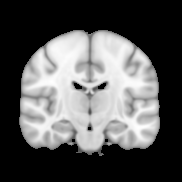
\includegraphics[width=5cm, height=8.5cm]{data/mri.png}
    };
    \draw[fill=black] (input.north east) --
        ($ (input.north east) - (\mridepth, 0) $) --
        ($ (input.north west) - (\mridepth, 0) $) --
        (input.north west) -- cycle;
    \draw[fill=black] (input.north west) --
        ($ (input.north west) - (\mridepth, 0) $) --
        ($ (input.south west) - (\mridepth, 0) $) --
        (input.south west) -- cycle;
    \draw[] (input.north east) --
        ($ (input.north east) + (\mridepth, 0) $) --
        ($ (input.north west) + (\mridepth, 0) $) --
        (input.north west) -- cycle;
    \draw[]  ($ (input.north west) + (\mridepth, 0) $) --
        ($ (input.south west) + (\mridepth, 0) $) --
        (input.south west);
    \draw[] ($ (input.north east) + (\mridepth, 0) $) --
        ($ (input.south east) + (\mridepth, 0) $) --
        ($ (input.south west) + (\mridepth, 0) $);
    \node[
        anchor=south,
        align=center,
        font=\fontsize{32}{32}\linespread{0.8}\selectfont
    ] at ($ (input.north east) - (0, 0) $) {
        T1-weighted\\
        structural MRI
    };
}

\newcommand{\convside}[6]{
    \node[
        fill=#5,
        inner sep=0pt,
        outer sep=0pt,
        minimum width=#3,
        minimum height=#4,
        draw=black
    ] (#6) at (#1, #2) {};
}

\newcommand{\convtop}[4]{
    \draw[fill=#4,draw=black] #1 --
    ($ #1 + (#3, #3) $) --
    ($ #1 + (#3+#2, #3) $) --
    ($ #1 + (#2, 0) $);
}

\newcommand{\convfront}[3]{
    \draw[black, fill=#3] #1 --
                        ($ #1 + (1*#2, 1*#2) $) --
                        ($ #1 + (1*#2, 1*#2 - 2*#2) $) --
                        ($ #1 + (0, -2*#2) $);
}


\newcommand{\convchannel}[5]{
    \def\huemin{20}
    \def\huemax{80}
    \pgfmathsetmacro{\iterations}{#5-1}
    \foreach \i in {0,...,\iterations} {
        \pgfmathsetmacro{\hue}{int(random(\huemin, \huemax))}
        \convside{#1}{#2+\i*-0.75}{#3}{#4/#5}{black!\hue}{n\i0}
        %\convtop{($ (n00.north west) + (0.5*\i*#4/#5, 0.5*\i*#4/#5) $)}{#3}{0.5*#4/#5}{black!\hue}

        \foreach \j in {0,...,\iterations} {
            \pgfmathsetmacro{\innerhue}{int(random(\huemin, \huemax))}
            \ifnum\j=0
                \pgfmathsetmacro{\innerhue}{\hue}
            \fi
            \convfront{($ (n00.north east) + (0.5*\j*#4/#5, 0.5*\j*#4/#5 - \i*#4/#5) $)}{0.5*#4/#5}{black!\innerhue}

            \ifnum\i=0
                \convtop{($ (n\i0.north west) + (0.5*\j*#4/#5, 0.5*\j*#4/#5) $)}{#3}{0.5*#4/#5}{black!\innerhue}
            \fi
        }
    }
}

\newcommand{\convlayer}[6]{
    \pgfmathsetmacro{\iterations}{#6-1}
    \foreach \i in {0,...,\iterations}{
        \pgfmathsetmacro{\x}{#1 + \i * 0.33}
        \convchannel{\x}{#2}{#3}{#4}{#5}
    }
}

\newcommand{\cnnarrow}[2]{
    \begin{scope}[transparency group, opacity=1]%0.5]
        \draw[-stealth, line width=15pt,red] #1 -- #2;
    \end{scope}
}

\newcommand{\cnn}[2]{
    \convlayer{#1}{#2-0.25}{0.33cm}{9cm}{12}{3}
    \cnnarrow{(#1 + 3.07, #2 - 2.1)}{(#1+7.5, #2 - 2.1)}
    \convlayer{#1 + 6.4}{#2-1}{0.33cm}{6cm}{8}{5}
    \cnnarrow{(#1 + 9.37, #2 - 2.1)}{(#1+13, #2 - 2.1)}
    \convlayer{#1 + 11.9}{#2-1.75}{0.33cm}{3cm}{4}{7}
    \cnnarrow{(#1 + 14.8, #2 - 2.1)}{(#1+18, #2 - 2.1)}
    \convlayer{#1 + 16.5}{#2-2.1}{0.33cm}{1.5cm}{2}{9}
    \cnnarrow{(#1 + 19.67, #2 - 2.1)}{(#1+22.2, #2 - 2.1)}

    \draw[thick, dashed] (#1 - 0.7, #2 + 5.1) --
                        (#1 + 20.6, #2 + 5.1) --
                        (#1 + 20.6, #2 - 9.4) --
                        (#1 - 0.7, #2 - 9.4) -- cycle;
    \node[anchor=south, text depth=0, font=\fontsize{32}{32}] at (#1 + 9.95, #2 + 5.1) {
        \textbf{3D Convolutional Neural Network}
    };
}

\newcommand{\lrpchannel}[5]{
    \def\huemin{30}
    \def\huemax{210}
    \colorlet{bgcolor}{black!90}
    \pgfmathsetmacro{\iterations}{#5-1}
    \foreach \i in {0,...,\iterations} {
        \pgfmathsetmacro{\red}{int(random(-150, 100))}
        \colorlet{fillcolor}{bgcolor}

        \ifnum\red>0
            \colorlet{fillcolor}{red!\red!bgcolor}
        \fi

        \convside{#1}{#2+\i*-0.75}{#3}{#4/#5}{fillcolor}{n\i0}
        %\convtop{($ (n00.north west) + (0.5*\i*#4/#5, 0.5*\i*#4/#5) $)}{#3}{0.5*#4/#5}{fillcolor}

        \foreach \j in {0,...,\iterations} {
            \pgfmathsetmacro{\innerred}{int(random(-150, 100))}
            \colorlet{innerfillcolor}{bgcolor}

            \ifnum\innerred>0
                \colorlet{innerfillcolor}{red!\innerred!bgcolor}
            \fi

            \ifnum\j=0
                \colorlet{innerfillcolor}{fillcolor}
            \fi

            \convfront{($ (n00.north east) + (0.5*\j*#4/#5, 0.5*\j*#4/#5 - \i*#4/#5) $)}{0.5*#4/#5}{innerfillcolor}
            \ifnum\i=0
                \convtop{($ (n\i0.north west) + (0.5*\j*#4/#5, 0.5*\j*#4/#5) $)}{#3}{0.5*#4/#5}{innerfillcolor}
            \fi
        }
    }
}

\newcommand{\lrplayer}[6]{
    \pgfmathsetmacro{\iterations}{#6-1}
    \foreach \i in {0,...,\iterations}{
        \pgfmathsetmacro{\x}{#1 + \i * 0.33}
        \lrpchannel{\x}{#2}{#3}{#4}{#5}
    }
}

\newcommand{\lrp}[2]{

    \lrplayer{#1}{#2-1}{0.33cm}{1.5cm}{2}{9}
    \cnnarrow{(#1 + 3.18, #2 - 1)}{(#1+6, #2 - 1)}
    \lrplayer{#1+4.55}{#2-0.65}{0.33cm}{3cm}{4}{7}
    \cnnarrow{(#1 + 7.45, #2 - 1)}{(#1+13, #2 - 1)}
    \lrplayer{#1 + 9.25}{#2+0.1}{0.33cm}{6cm}{8}{5}
    \cnnarrow{(#1 + 12.23, #2 - 1)}{(#1+20, #2 - 1)}
    \lrplayer{#1 + 14.85}{#2 + 0.85}{0.33cm}{9cm}{12}{3}

    \draw[thick, dashed] (#1 - 0.7, #2 + 6.25) --
                        (#1 + 20.6, #2 + 6.25) --
                        (#1 + 20.6, #2 - 8.25) --
                        (#1 - 0.7, #2 - 8.25) -- cycle;
    \node[anchor=south, text depth=0, font=\fontsize{32}{32}] at (#1 + 9.95, #2 + 6.25) {
        \textbf{Layerwise relevance propagation}
    };
}

\newcommand{\heatmap}[2]{
    \node[yslant=1, inner sep=0pt] (map) at (#1, #2) {
        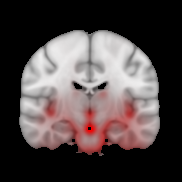
\includegraphics[width=5cm, height=8.5cm]{data/heatmap.png}
    };
    \draw[fill=black] (map.north east) --
        ($ (map.north east) - (\mridepth, 0) $) --
        ($ (map.north west) - (\mridepth, 0) $) --
        (map.north west) -- cycle;
    \draw[fill=black] (map.north west) --
        ($ (map.north west) - (\mridepth, 0) $) --
        ($ (map.south west) - (\mridepth, 0) $) --
        (map.south west) -- cycle;
    \draw[] (map.north east) --
        ($ (map.north east) + (\mridepth, 0) $) --
        ($ (map.north west) + (\mridepth, 0) $) --
        (map.north west) -- cycle;
    \draw[]  ($ (map.north west) + (\mridepth, 0) $) --
        ($ (map.south west) + (\mridepth, 0) $) --
        (map.south west);
    \draw[] ($ (map.north east) + (\mridepth, 0) $) --
        ($ (map.south east) + (\mridepth, 0) $) --
        ($ (map.south west) + (\mridepth, 0) $);
    \node[
        anchor=south,
        align=center,
        font=\fontsize{32}{32}\linespread{0.8}\selectfont
    ] at (map.north east) {
        Explanatory\\
        heatmaps
    };
}


\begin{figure}[h]
    \begin{tikzpicture}
        \mriinput{-1.2}{-1.15}

        \cnnarrow{(-1.2, -1.15)}{(7, -1.15)}

        \cnn{6}{1}

        \node[align=center,font=\fontsize{32}{32}] at (34, -1.15) {
            \textit{Predicted probability}\\\textit{of dementia}
        };
        \cnnarrow{(39.7, -1.15)}{(53, -1.15)}

        \lrp{41.5}{-0.15}
        \cnnarrow{(59.43, -1.15)}{(67, -1.15)}

        \heatmap{68.6}{-1.15}
    \end{tikzpicture}
\end{figure}
